\documentclass{article}
\PassOptionsToPackage{numbers,compress}{natbib}
\usepackage[final]{neurips}

\usepackage[utf8]{inputenc}
\usepackage[T1]{fontenc}
\usepackage{amsmath}
\usepackage{booktabs}
\usepackage{graphicx}
\usepackage{hyperref}
\hypersetup{hidelinks}

\setlength{\textfloatsep}{7pt plus 2pt minus 2pt}
\setlength{\intextsep}{6pt plus 2pt minus 2pt}

\title{Few-Shot Day-to-Night Translation: Paired vs. Unpaired Supervision}

\author{%
  Yuxin Chen \quad Chen Hao Zhang \quad Meixuan Chen\\
  Department of Electrical \& Computer Engineering, University of Toronto\\
  \texttt{\{katy.chen, chenhao.zhang, meixan.chen\}@mail.utoronto.ca}
}

\begin{document}
\maketitle

\begin{abstract}
We compare paired and unpaired supervision for few-shot day-to-night driving-scene translation using pix2pix-turbo and CycleGAN-Turbo, two one-step models built on SD-Turbo. We train each model with 5, 10, 20, and 50 examples using three seeds, then evaluate the same 200 held-out pairs with SSIM, LPIPS, CLIP similarity, and CMMD. pix2pix-turbo consistently achieves lower LPIPS, whereas CycleGAN-Turbo achieves lower CMMD, revealing a trade-off between paired-target perceptual fidelity and distributional alignment. No adjacent-shot candidate survives Holm correction under our pre-specified breaking-point criterion. Unadjusted exploratory screens instead place pix2pix-turbo instability at 5 shots on LPIPS and CLIP similarity, while CycleGAN-Turbo shows CLIP instability at 10 shots and additional LPIPS/CLIP degradation at 5 shots. With only three seeds, these signals should not be interpreted as definitive thresholds.
\end{abstract}

\section*{Statement of Teamwork}
The success of this report relies on the joint effort of all team members. Yuxin Chen and Chen Hao Zhang contributed to the implementation of the training and evaluation pipelines for pix2pix-Turbo and CycleGAN-Turbo respectively. Meixuan Chen contributed to the data preparation, qualitative and quantitative evaluation of the models. All team members participated in discussions and decision-making throughout the project, including the design of the experimental protocol and the interpretation of the results, and also the writing of the report.

\section{Introduction}

Day-to-night translation can expand driving data across illumination conditions, but paired examples are costly to collect. Paired methods can directly imitate a target transformation, while unpaired methods trade correspondence for domain-level supervision. This distinction is especially consequential when only a handful of images are available.

We ask: (1) which supervision paradigm learns day-to-night translation more effectively at 5--50 shots, and (2) at which shot level does performance become statistically unstable? We contribute a controlled $2$-model $\times$ $4$-shot $\times$ $3$-seed comparison, a fixed held-out evaluation protocol, and an explicit breaking-point analysis that separates mean degradation from seed- and sample-level variability.

\section{Related Work and Model Architecture}

Classical pix2pix learns a conditional generator from aligned input--target pairs using a conditional discriminator and direct reconstruction loss \cite{isola2017image}. CycleGAN removes the pairing requirement by learning mappings in both directions with domain discriminators and cycle consistency; identity loss further discourages unnecessary changes to samples already in the target domain \cite{zhu2017unpaired}. These methods motivate the paired and unpaired objectives studied here, but their original convolutional generators do not exploit a pretrained text-to-image prior.

img2img-turbo instead adapts the distilled SD-Turbo model into an end-to-end, one-step image translator \cite{parmar2024one,sauer2023adversarial}. An input image is encoded by the VAE, its latent replaces the usual initial diffusion noise, and a text-conditioned U-Net makes one prediction at the terminal diffusion timestep before the VAE decoder reconstructs the output. LoRA adapters provide parameter-efficient updates \cite{hu2021lora}; trainable zero-convolution skip paths carry multi-scale encoder activations directly to the decoder to preserve spatial detail, and the U-Net input convolution is also adapted. The pretrained text encoder and most backbone weights remain frozen.

pix2pix-turbo applies this generator once from day to night. Its released training objective combines paired pixel and LPIPS reconstruction, generated-image--target-text CLIP alignment, and a vision-aided adversarial loss on real versus generated target-domain images. CycleGAN-Turbo applies the same shared one-step U-Net in both directions, selected by day/night text embeddings, while using direction-specific VAE adaptation paths. Two discriminators enforce day and night realism; $x\!\rightarrow\!\hat y\!\rightarrow\!x_{\mathrm{rec}}$ and $y\!\rightarrow\!\hat x\!\rightarrow\!y_{\mathrm{rec}}$ receive L1 and LPIPS cycle losses, and identity passes receive analogous penalties. Thus, CycleGAN-Turbo does not use aligned day/night targets even when such filenames exist.

The released pix2pix-turbo interface also supports stochastic generation by interpolating the encoded input with an external noise map and scaling adapters with a parameter $r$; CycleGAN-Turbo exposes no analogous interpolation control, although both implementations sample a VAE posterior latent. We did not tune these diversity controls. Formal evaluation used the pix2pix default deterministic branch, a fixed prompt, and a deterministic per-filename RNG seed for both models. Each primary score therefore represents one reproducible output per checkpoint and input, so breaking-point variability concerns training seeds and test samples. A separate repeated-generation diagnostic in Appendix~\ref{app:inference-variability} measures residual inference-seed sensitivity.

\section{Methods}

\subsection{Models and Objectives}

Our implementation retains the architecture and losses above but matches adaptation capacity across models. The released training code defaults to U-Net LoRA rank 8 for pix2pix-turbo and 128 for CycleGAN-Turbo, VAE rank 4, learning rate $5\times10^{-6}$, and batch size 4. We instead use U-Net/VAE ranks 32/4 for both models, learning rate $10^{-5}$, batch size 1, and a fixed 2,000-step budget selected through held-out pilot experiments. Their objectives can be summarized as
\begin{align}
\mathcal{L}_{\mathrm{pix}}
  &= \lambda_{2}\mathcal{L}_{2}
   + \lambda_{\mathrm{LPIPS}}\mathcal{L}_{\mathrm{LPIPS}}
   + \lambda_{\mathrm{CLIP}}\mathcal{L}_{\mathrm{CLIP}}
   + \lambda_{\mathrm{GAN}}\mathcal{L}_{\mathrm{GAN}}, \\
\mathcal{L}_{\mathrm{cycle}}
  &= \lambda_{\mathrm{cyc},1}\mathcal{L}_{\mathrm{cyc},1}
   + \lambda_{\mathrm{cyc},p}\mathcal{L}_{\mathrm{cyc},p}
   + \lambda_{\mathrm{id},1}\mathcal{L}_{\mathrm{id},1} \notag \\
  &\quad
   + \lambda_{\mathrm{id},p}\mathcal{L}_{\mathrm{id},p}
   + \lambda_{\mathrm{GAN}}\mathcal{L}_{\mathrm{GAN}}.
\end{align}
The comparison therefore shares the SD-Turbo backbone and LoRA ranks while retaining the supervision-specific objectives. Exact component weights and runtime settings are listed in Appendix~\ref{app:settings}.

\subsection{Data and Training Protocol}

We use DarkDriving \cite{wang2026darkdriving}, whose raw release contains 5,906 aligned training pairs and 3,632 held-out pairs. Both images in each pair were fully decoded before sampling; six corrupted training pairs and two corrupted test pairs were excluded, leaving 5,900 and 3,630 valid pairs. We reserved 100 training pairs for pilot hyperparameter and checkpoint selection, never using the held-out test set for tuning. Few-shot splits were sampled from the remaining pool using the experiment seed and were nested within each seed: $5\subset10\subset20\subset50$. The 5-shot condition was added post hoc as an exploratory extension to the original 10/20/50-shot grid. The breaking-point criterion was fixed before running the 5-shot extension.

Every run used AdamW, learning rate $10^{-5}$, batch size 1, resolution $512\times512$, 2,000 optimizer steps, and seed 1, 2, or 3 on a single NVIDIA RTX 5090. This fixes the stopping budget but not computation per step or effective epochs. Architecture-specific precision and memory settings were retained for stability. CycleGAN-Turbo checkpoints explicitly include the trainable U-Net \texttt{conv\_in} weights in addition to LoRA and VAE weights.

\subsection{Controlled Evaluation and Breaking Point}

Formal evaluation used one deterministic 200-pair subset sampled from the valid held-out split with seed 42 and reused for every condition. Generation used base seed 0 plus a deterministic filename-derived seed, making outputs independent of traversal order. Manifests enforced identical filenames across runs. We report per-image SSIM \cite{wang2004image}, LPIPS with AlexNet, and CLIP image-image similarity with ViT-B/32 \cite{radford2021learning}. Following the official CMMD reference implementation, we use normalized ViT-L/14@336px image embeddings, a Gaussian kernel with $\sigma=10$, the minimum-variance biased estimator, and the conventional $1000\times$ reporting scale \cite{jayasumana2024rethinking}. Higher SSIM and CLIP are better; lower LPIPS and CMMD are better.

For adjacent shot levels $L<H$, a metric-specific breaking point requires: (i) worse mean performance at $L$ under a one-sided, seed-ID-paired $t$-test; (ii) a between-seed variance ratio $\operatorname{Var}(L)/\operatorname{Var}(H)>1$; and, for per-image metrics, (iii) an analogous test-sample variance ratio above 1. Holm correction controls 12 adjacent-shot tests per model (four metrics across three transitions); we call a result confirmed only when the adjusted $p<0.05$. CMMD is dataset-level, so sample variance is not applicable. With only three seeds, effect sizes and variance ratios remain essential context.

\section{Results}

\subsection{Overall Performance}

Most mean improvements occur between 5 and 20 shots (Figure~\ref{fig:performance}). Beyond 20 shots, LPIPS and CLIP similarity largely plateau; CMMD improves modestly for pix2pix-turbo and slightly worsens for CycleGAN-Turbo at 50 shots. SSIM is less stable: pix2pix-turbo peaks at 20 shots and declines at 50, while CycleGAN-Turbo continues to improve. Across every shot level, pix2pix-turbo has lower LPIPS and CycleGAN-Turbo has lower CMMD, although the CMMD gap is negligible at 50 shots. This pattern is consistent with the supervision objectives: paired reconstruction rewards similarity to a specific nighttime target, whereas independent-domain cycle training rewards matching the nighttime distribution without reproducing that target exactly. SSIM and CLIP are broadly comparable at 20--50 shots, so neither model dominates all notions of quality.

\subsection{Breaking-Point Analysis}

\begin{table}[h]
  \caption{Strongest exploratory breaking-point candidates. Variance ratios are seed/sample; none remains significant after Holm correction.}
  \label{tab:breaking}
  \centering
  \small
  \setlength{\tabcolsep}{4pt}
  \begin{tabular}{lccccc}
    \toprule
    Model & Comparison & Evidence & Degradation & Variance ratios & Raw / Holm $p$ \\
    \midrule
    pix2pix-turbo  & 5 vs 10  & CLIP  & $0.0293$ lower & $5.81/1.41\times$ & .016 / .177 \\
    pix2pix-turbo  & 5 vs 10  & LPIPS & $+0.0258$ & $88.15/1.28\times$ & .032 / .322 \\
    CycleGAN-Turbo & 10 vs 20 & CLIP  & $0.0122$ lower & $42.16/1.25\times$ & .004 / .051 \\
    CycleGAN-Turbo & 5 vs 10  & LPIPS & $+0.0429$ & $9.38/1.53\times$ & .007 / .075 \\
    \bottomrule
  \end{tabular}
\end{table}

No transition meets the Holm-confirmed criterion (Table~\ref{tab:breaking}). Before multiplicity correction, pix2pix-turbo shows 5-shot degradation on LPIPS and CLIP similarity, each with increased seed and sample variance. CycleGAN-Turbo shows CLIP degradation from 10 to 20 shots---the earliest instability encountered as supervision is reduced---plus LPIPS and CLIP degradation from 5 to 10 shots. The 10-shot CLIP candidate is closest to confirmation (Holm $p=0.0507$), but remains exploratory. CycleGAN-Turbo's 5-shot SSIM mean also degrades (raw $p=0.0049$), yet its sample variance ratio is $0.98$, so it fails the complete criterion.

\subsection{Qualitative Comparison}

Figure~\ref{fig:qualitative} illustrates the metric-dependent behavior. Five-shot outputs show stronger changes in lighting and appearance, while the 10- and 50-shot outputs are generally more stable. pix2pix-turbo tends to remain closer to the paired nighttime target; CycleGAN-Turbo more freely changes global illumination, consistent with the LPIPS/CMMD trade-off. After quantitative analysis, typical was selected nearest the median aggregate per-image difficulty and breaking-sensitive to maximize the selected low-shot degradations. CMMD was excluded because it has no per-image value. These post-hoc examples illustrate, but do not independently validate, the fixed 200-image quantitative results.

\section{Discussion and Limitations}

In this comparison, pix2pix-turbo achieves better paired-target fidelity, as reflected by lower LPIPS, whereas CycleGAN-Turbo achieves better distributional alignment under our distribution-level metric. Because the models differ in their objectives and some implementation settings, these differences should not be attributed to supervision alone. At 20--50 shots, the models converge on similar SSIM and CLIP values while retaining this fidelity--distribution trade-off. The practical choice should therefore follow the intended criterion rather than a universal model ranking. The absence of a Holm-confirmed threshold is itself informative: the observed low-shot changes are metric-specific and too uncertain to support a single universal breaking point.

Six limitations constrain interpretation. First, three seeds provide limited statistical power, so even the near-threshold Holm result is uncertain. Second, results cover one driving dataset, one backbone, and one set of loss weights. Third, the fixed 2,000-step budget equalizes stopping but not effective epochs or compute. Fourth, CMMD is distribution-level and has no per-sample variance. Fifth, the inference-seed diagnostic covers only one 10-shot checkpoint and does not test pix2pix-turbo's explicit stochastic interpolation parameter. Finally, one model represents each supervision regime, so model-specific architectural and objective differences are confounded with the paired-versus-unpaired comparison. Additional seeds, datasets, broader repeated-generation sweeps, and training-budget sweeps are needed before assigning a general breaking threshold. 

\section{Conclusion}

Few-shot robustness is metric-specific, and no adjacent-shot transition is Holm-confirmed as a breaking point. Unadjusted evidence suggests pix2pix-turbo becomes unstable at 5 shots, while CycleGAN-Turbo may show earlier CLIP instability at 10 shots. Most gains arrive by 20 shots; thereafter, LPIPS and CLIP largely plateau while SSIM and CMMD remain model- and seed-sensitive. Paired pix2pix-turbo favors target fidelity, whereas unpaired CycleGAN-Turbo favors distributional alignment.

\begin{figure}[p]
  \centering
  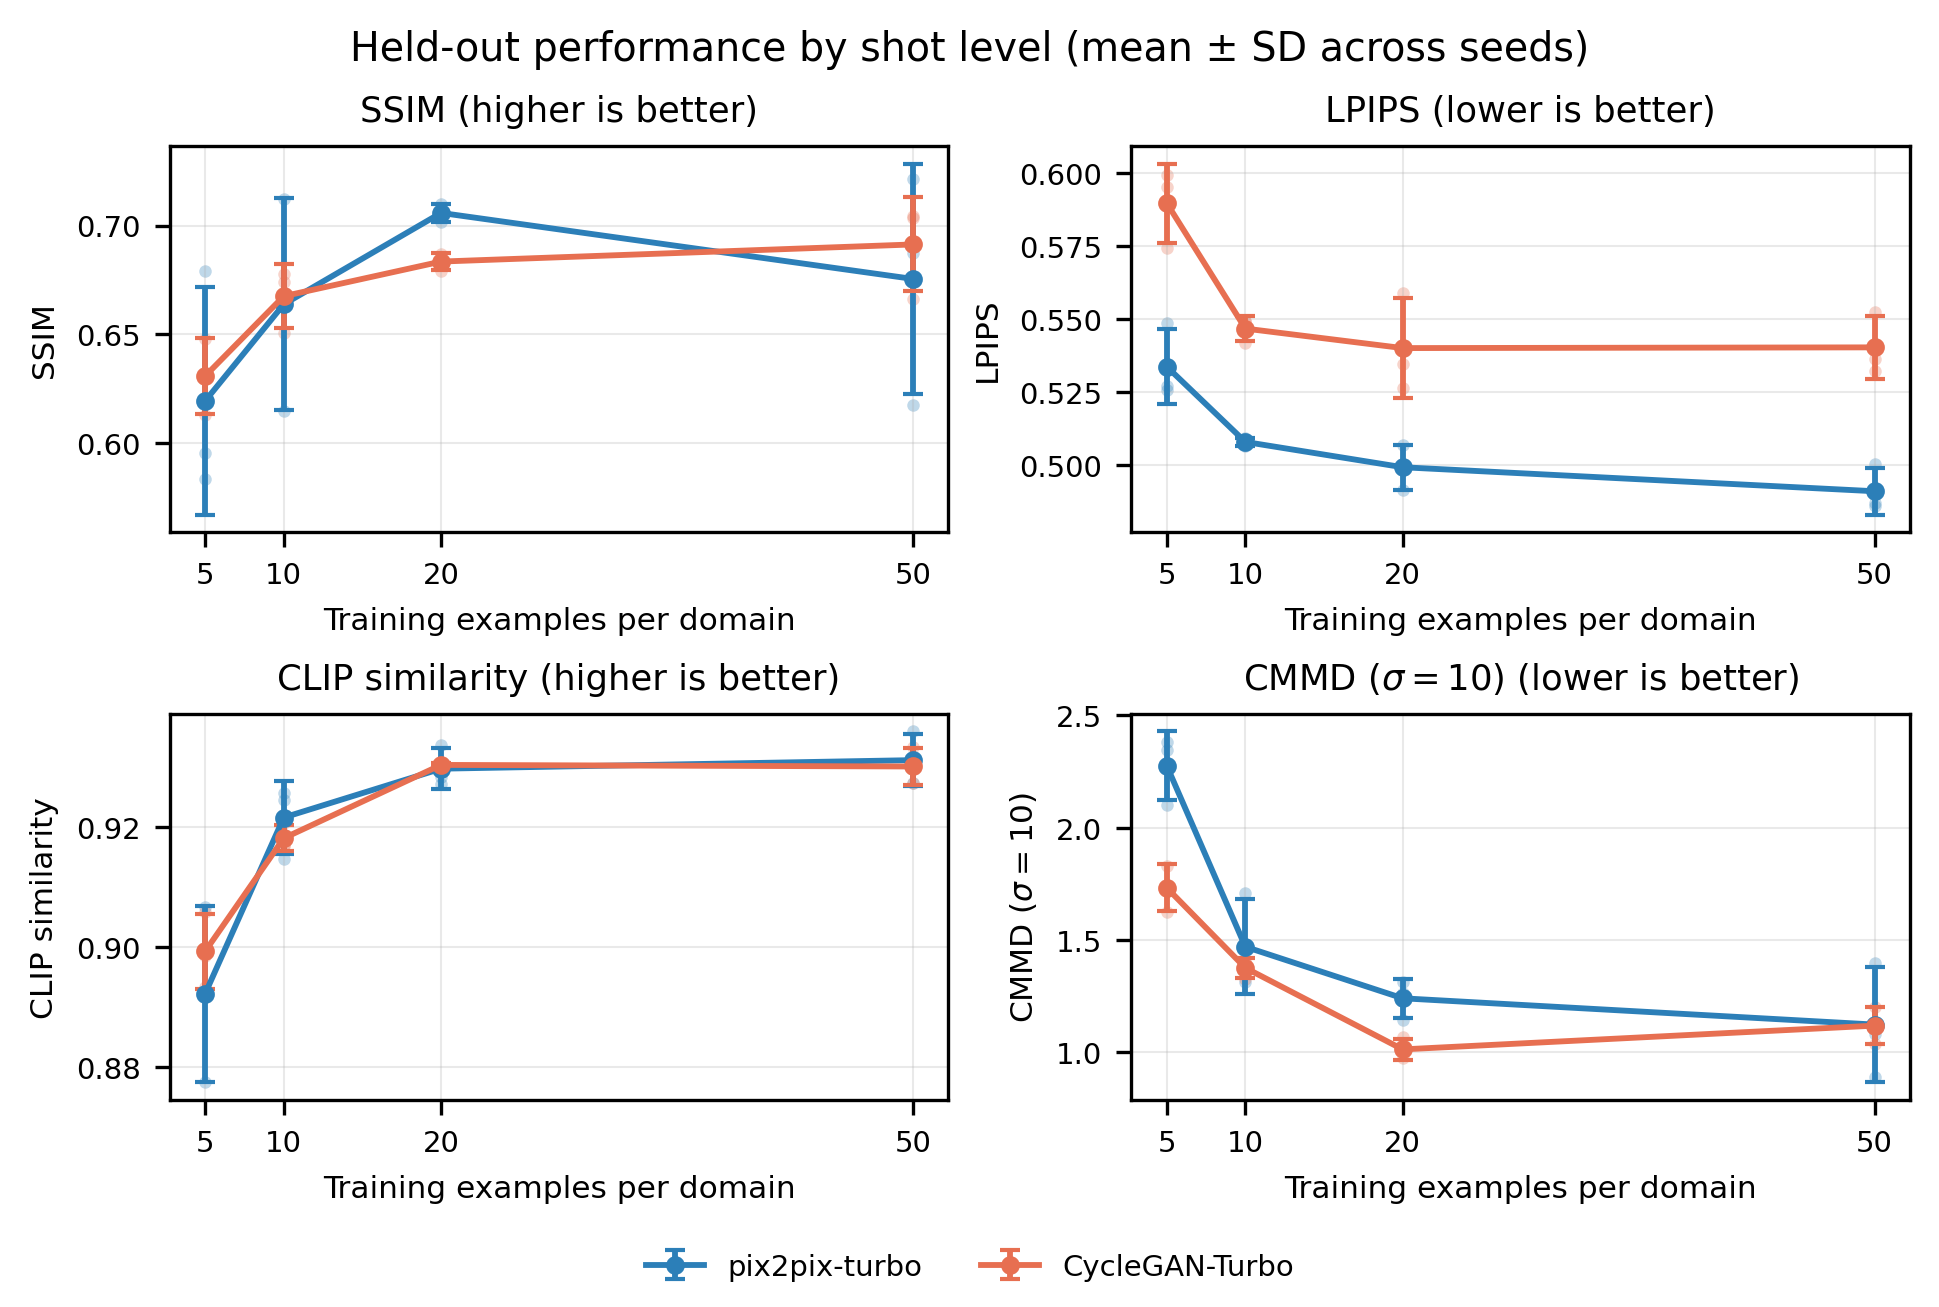
\includegraphics[width=0.68\textwidth]{figures/performance_by_shot.png}
  \caption{Held-out performance across shot levels. Large markers show means and bars show one standard deviation across three seeds; faint points show individual seeds. Exact means appear in Appendix~\ref{app:means}.}
  \label{fig:performance}
\end{figure}

\begin{figure}[p]
  \centering
  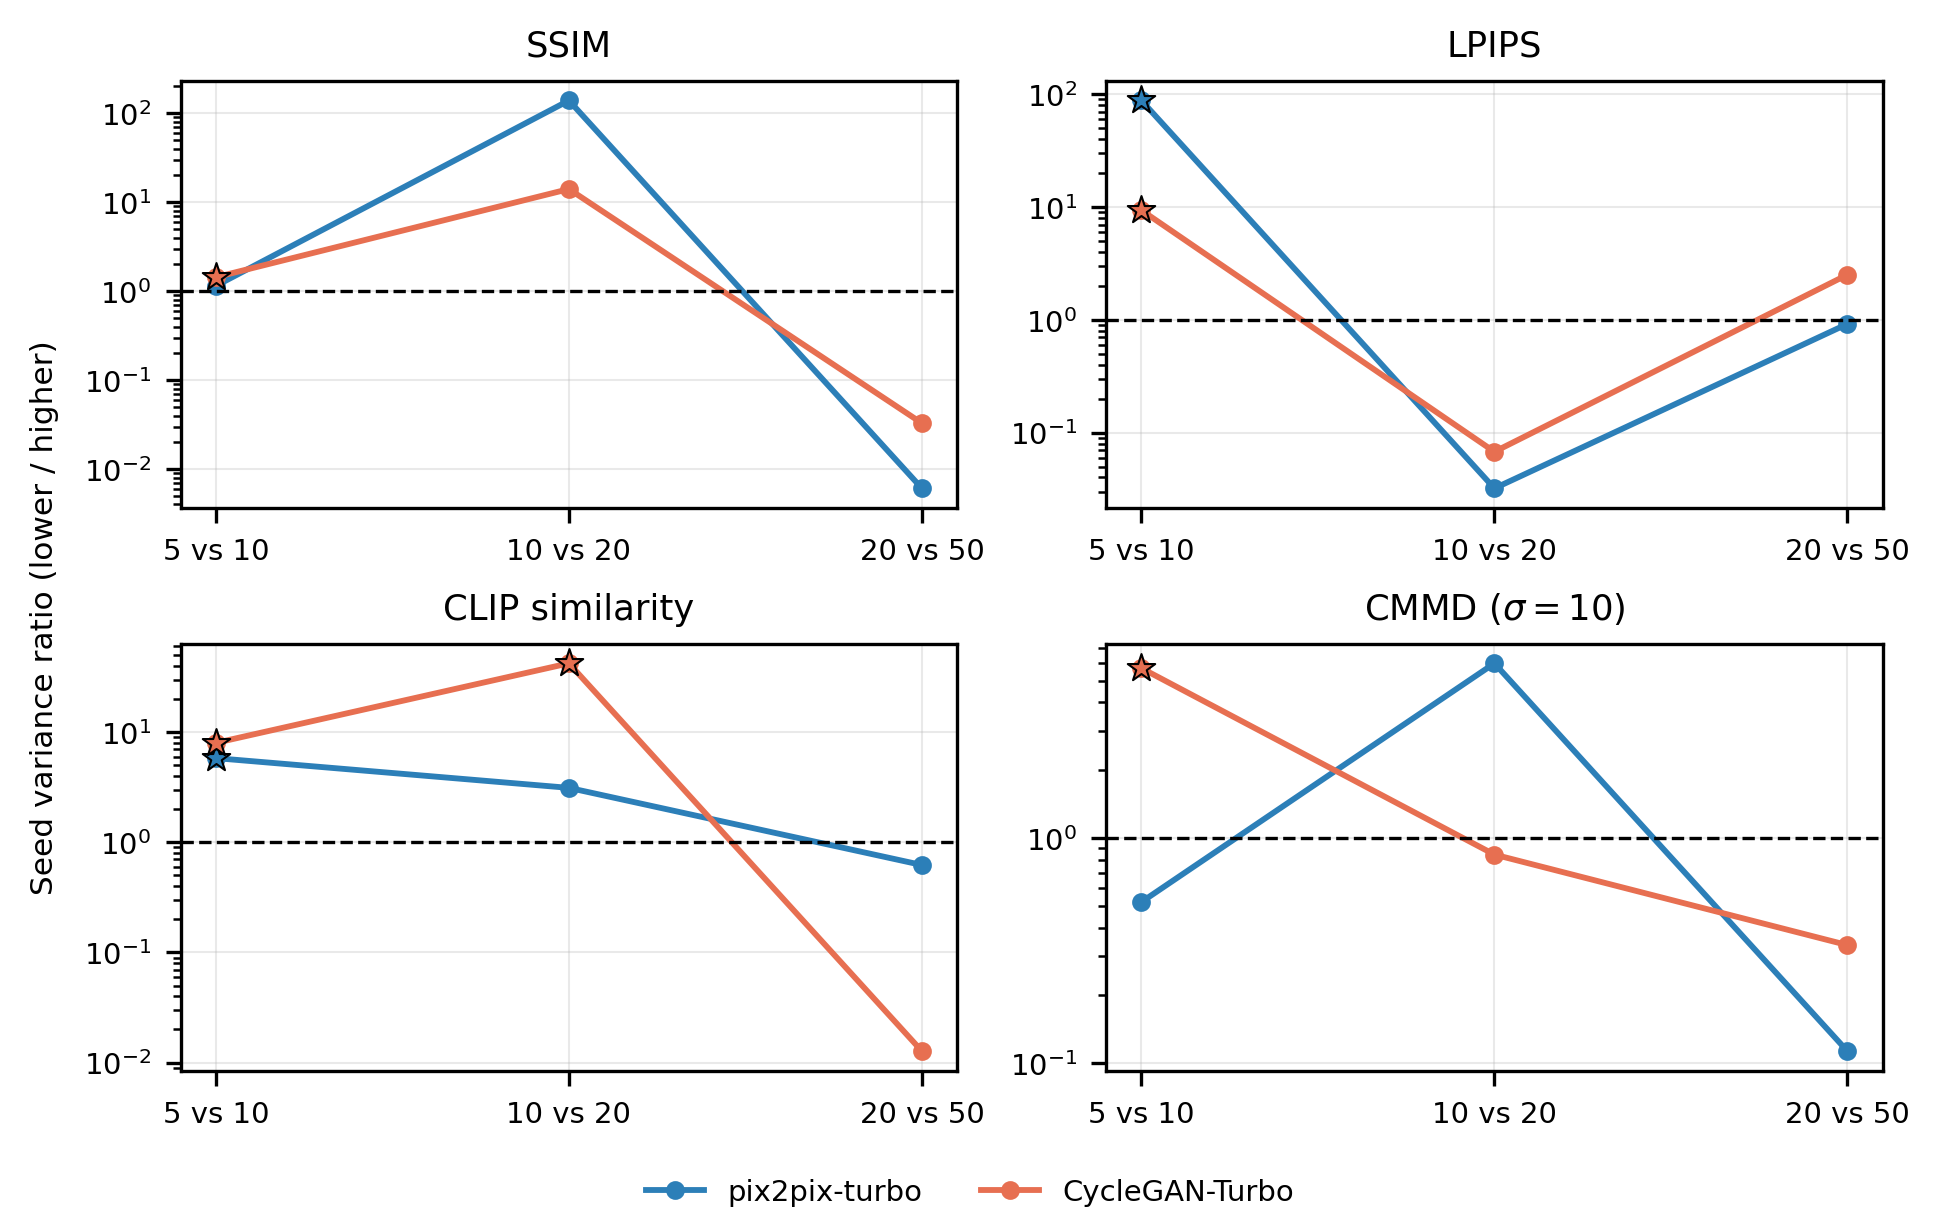
\includegraphics[width=0.68\textwidth]{figures/instability_by_shot.png}
  \caption{Between-seed variance ratios for adjacent shot levels. The dashed line marks equal variance. Stars identify raw-significant mean degradation with increased seed variance; formal confirmation additionally requires increased test-sample variance and Holm-adjusted significance.}
  \label{fig:instability}
\end{figure}

\begin{figure}[p]
  \centering
  \includegraphics[width=0.98\textwidth]{../results/qualitative_figures/qualitative_slide_compact.png}
  \caption{Fixed held-out scenes at training seed 1 and filename-stable inference seed 0. Cases were selected post hoc using quantitative rules rather than visual preference.}
  \label{fig:qualitative}
\end{figure}

\clearpage
\small
\begin{thebibliography}{10}

\bibitem{parmar2024one}
Parmar, G., Park, T., Narasimhan, S., \& Zhu, J.-Y. (2024). One-Step Image Translation with Text-to-Image Models. \textit{arXiv:2403.12036}.

\bibitem{isola2017image}
Isola, P., Zhu, J.-Y., Zhou, T., \& Efros, A. A. (2017). Image-to-Image Translation with Conditional Adversarial Networks. \textit{CVPR}.

\bibitem{zhu2017unpaired}
Zhu, J.-Y., Park, T., Isola, P., \& Efros, A. A. (2017). Unpaired Image-to-Image Translation using Cycle-Consistent Adversarial Networks. \textit{ICCV}.

\bibitem{zhang2018unreasonable}
Zhang, R., Isola, P., Efros, A. A., Shechtman, E., \& Wang, O. (2018). The Unreasonable Effectiveness of Deep Features as a Perceptual Metric. \textit{CVPR}.

\bibitem{sauer2023adversarial}
Sauer, A., Lorenz, D., Blattmann, A., \& Rombach, R. (2023). Adversarial Diffusion Distillation. \textit{arXiv:2311.17042}.

\bibitem{hu2021lora}
Hu, E. J., et al. (2021). LoRA: Low-Rank Adaptation of Large Language Models. \textit{ICLR}.

\bibitem{wang2026darkdriving}
Wang, W., et al. (2026). DarkDriving: A Real-World Day and Night Aligned Dataset for Autonomous Driving in the Dark Environment. \textit{arXiv:2603.18067}.

\bibitem{wang2004image}
Wang, Z., Bovik, A. C., Sheikh, H. R., \& Simoncelli, E. P. (2004). Image Quality Assessment: From Error Visibility to Structural Similarity. \textit{IEEE TIP}.

\bibitem{radford2021learning}
Radford, A., et al. (2021). Learning Transferable Visual Models From Natural Language Supervision. \textit{ICML}.

\bibitem{jayasumana2024rethinking}
Jayasumana, S., et al. (2024). Rethinking FID: Towards a Better Evaluation Metric for Image Generation. \textit{CVPR}.

\end{thebibliography}

\clearpage
\appendix
\normalsize

\section{Complete Experimental Settings}
\label{app:settings}

\begin{table}[h]
  \caption{Shared and architecture-specific training settings.}
  \centering
  \small
  \setlength{\tabcolsep}{7pt}
  \begin{tabular}{lll}
    \toprule
    Setting & pix2pix-turbo & CycleGAN-Turbo \\
    \midrule
    Backbone & SD-Turbo & SD-Turbo \\
    Optimizer / learning rate & AdamW / $10^{-5}$ & AdamW / $10^{-5}$ \\
    Resolution / batch size & $512\times512$ / 1 & $512\times512$ / 1 \\
    Optimizer steps & 2,000 & 2,000 \\
    U-Net / VAE LoRA rank & 32 / 4 & 32 / 4 \\
    Precision & full precision & FP16 \\
    Gradient checkpointing & disabled & enabled \\
    Data-loader workers & 4 & 0 \\
    Training preparation & resized crop & direct resize \\
    Held-out preparation & direct resize & direct resize \\
    \bottomrule
  \end{tabular}
\end{table}

\begin{table}[h]
  \caption{Loss weights used in the formal grid. A dash denotes a component not used by that model.}
  \centering
  \small
  \setlength{\tabcolsep}{7pt}
  \begin{tabular}{lcc}
    \toprule
    Component & pix2pix-turbo & CycleGAN-Turbo \\
    \midrule
    L2 reconstruction & 1.0 & -- \\
    LPIPS / cycle LPIPS & 5.0 & 10.0 \\
    CLIP image-text & 5.0 & -- \\
    Cycle L1 & -- & 1.0 \\
    Identity L1 / LPIPS & -- & 1.0 / 1.0 \\
    GAN & 0.5 & 0.5 \\
    \bottomrule
  \end{tabular}
\end{table}

The source and target prompts were fixed as ``a driving scene during the day'' and ``a driving scene during the night.'' Generation used base seed 0 and a deterministic filename-derived seed. All 24 conditions used the same 200 held-out filenames. For CycleGAN-Turbo, checkpoint save/load additionally preserves the trainable U-Net \texttt{conv\_in} parameters; omitting them changes inference despite loading the LoRA and VAE components.

\section{Complete Quantitative Means}
\label{app:means}

\begin{table}[h]
  \caption{Held-out mean $\pm$ sample standard deviation across three training seeds.}
  \centering
  \scriptsize
  \setlength{\tabcolsep}{3pt}
  \begin{tabular}{lccccc}
    \toprule
    Model & Shots & SSIM $\uparrow$ & LPIPS $\downarrow$ & CLIP $\uparrow$ & CMMD $\downarrow$ \\
    \midrule
    CycleGAN-Turbo & 5  & $0.6309\pm0.0175$ & $0.5896\pm0.0135$ & $0.8993\pm0.0062$ & $1.7325\pm0.1044$ \\
                   & 10 & $0.6676\pm0.0146$ & $0.5467\pm0.0044$ & $0.9181\pm0.0022$ & $1.3760\pm0.0438$ \\
                   & 20 & $0.6835\pm0.0039$ & $0.5400\pm0.0170$ & $0.9303\pm0.0003$ & $1.0134\pm0.0477$ \\
                   & 50 & $0.6913\pm0.0216$ & $0.5403\pm0.0107$ & $0.9300\pm0.0030$ & $1.1192\pm0.0825$ \\
    \midrule
    pix2pix-turbo  & 5  & $0.6194\pm0.0521$ & $0.5337\pm0.0128$ & $0.8922\pm0.0146$ & $2.2759\pm0.1520$ \\
                   & 10 & $0.6638\pm0.0486$ & $0.5079\pm0.0014$ & $0.9215\pm0.0061$ & $1.4699\pm0.2110$ \\
                   & 20 & $0.7058\pm0.0041$ & $0.4993\pm0.0076$ & $0.9297\pm0.0034$ & $1.2408\pm0.0864$ \\
                   & 50 & $0.6755\pm0.0529$ & $0.4911\pm0.0080$ & $0.9311\pm0.0044$ & $1.1238\pm0.2571$ \\
    \bottomrule
  \end{tabular}
\end{table}

\clearpage
\section{Additional Qualitative Case}

\begin{figure}[h]
  \centering
  \includegraphics[width=\textwidth]{../results/qualitative_figures/qualitative_all_cases.png}
  \caption{Expanded qualitative comparison including post-hoc typical, challenging, and breaking-sensitive cases selected by quantitative rules. Conditions use training seed 1 and identical filenames with inference seed 0.}
  \label{fig:qualitative-full}
\end{figure}

\section{Reproducibility Protocol}

After integrity filtering, each training split was sampled from the same valid pool using its experiment seed. For evaluation, generation manifests recorded every filename and seed, and the evaluator rejected mismatched generated/target pairs. The analysis proceeded as follows:
\begin{enumerate}
  \item train both models for each shot level and seed with a fixed 2,000-step stopping rule;
  \item generate the fixed 200-image held-out subset with filename-stable inference seeds;
  \item compute per-image SSIM, LPIPS, and CLIP similarity and per-run CMMD;
  \item aggregate first within each run, then across the three training seeds;
  \item perform seed-ID-paired adjacent-shot tests and Holm correction within each model; and
  \item use per-image variance only as a grouped, within-seed diagnostic rather than treating repeated images as independent training runs.
\end{enumerate}

Qualitative cases were selected from the same 200 filenames without inspecting the images. Define aggregate difficulty as standardized LPIPS minus standardized SSIM and CLIP similarity. The typical case is closest to its median, the challenging case is closest to its 90th percentile, and the breaking-sensitive case maximizes the pre-specified combination of pix2pix-turbo 5-to-10 LPIPS degradation and CycleGAN-Turbo 10-to-20 CLIP degradation, while favoring seed-consistent changes.

\clearpage
\section{Inference-Seed Sensitivity}
\label{app:inference-variability}

We additionally held the 10-shot, training-seed-1 checkpoint and 20 test inputs fixed while varying the inference seed from 0 to 4. For each input, we compared all ten unordered output pairs. Pairwise LPIPS measures perceptual change; MAE and the 95th-percentile absolute difference are reported in 8-bit intensity levels, and PSNR is computed directly between generated outputs. These quantities measure sensitivity rather than image quality.

\begin{table}[h]
  \caption{Repeated-generation sensitivity across 20 inputs and five inference seeds (200 output-pair comparisons per model). Lower LPIPS and pixel differences, higher PSNR, and more unchanged channels indicate lower sensitivity.}
  \centering
  \scriptsize
  \setlength{\tabcolsep}{4pt}
  \begin{tabular}{lccccc}
    \toprule
    Model & LPIPS $\downarrow$ & MAE $\downarrow$ & 95th pct. $\downarrow$ & PSNR $\uparrow$ & Unchanged \%
    \\
    \midrule
    pix2pix-turbo & 0.00996 & 0.2505 & 1.175 & 52.28 & 80.49 \\
    CycleGAN-Turbo & 0.00964 & 0.2432 & 1.115 & 52.33 & 81.14 \\
    \bottomrule
  \end{tabular}
\end{table}

No input produced byte-identical files across all five seeds, confirming numerical stochasticity. Nevertheless, pairwise LPIPS remained below 0.01 on average, mean absolute differences were about one quarter of an 8-bit level, and pairwise PSNR exceeded 52 dB for both models. We therefore characterize both as having low inference-seed sensitivity under the evaluated default inference paths. CycleGAN-Turbo's slightly smaller values are descriptive only: this diagnostic uses one checkpoint and was not designed or powered as a model-ranking test.

\end{document}
